\documentclass[11pt,a4paper]{article}

\usepackage[T1]{fontenc}
\usepackage[utf8]{inputenc}
\usepackage{lmodern}
\usepackage{amsmath,amssymb,amsfonts,bm}
\usepackage{booktabs}
\usepackage{array}
\usepackage{longtable}
\usepackage{geometry}
\usepackage{graphicx}
\usepackage{xcolor}
\usepackage{hyperref}
\usepackage{microtype}
\usepackage{enumitem}

\geometry{margin=1in}
\hypersetup{
  colorlinks=true,
  linkcolor=blue!50!black,
  citecolor=blue!50!black,
  urlcolor=blue!50!black
}
\setlist[itemize]{leftmargin=1.4em}
\setlist[enumerate]{leftmargin=1.6em}
\renewcommand{\arraystretch}{1.16}

\title{\textbf{Open Quantum Control Laboratory for Dissipative Spin-$3/2$ Dynamics:}\\
\large A Reproducible Review, Benchmark, and Experimental-Decision Framework}

\author{
Pedro Henrique, Ygor, and the Open Quantum Control working repository\\
\small Python-first computational laboratory for open quantum systems, NMR, tomography, and control
}

\date{Draft generated from the local reproducibility layer, April 2026}

\begin{document}

\maketitle

\begin{abstract}
This draft consolidates the current state of the Open Quantum Control laboratory:
a Python-first research environment designed to identify and control dissipative
quantum dynamics, initially through quadrupolar Na-23 nuclear magnetic resonance
(NMR) and then through hardware-facing characterization workflows.  The document
reviews the external papers reproduced so far, the internal physical benchmarks,
the mathematical model stack, the computational laboratory architecture, and the
new experimental-decision pipeline.  The central theme is the control and
identification of dissipative dynamics in open quantum systems with experimental
validation.  The technical strategy is deliberately reproducible: each paper
reproduction or workflow generates scripts, configuration files, figures,
metrics, hashes, and a local research-memory record.  The present stage is not a
claim of experimental confirmation.  It is a validated synthetic benchmark layer
that specifies what should be measured next, how incoming data should be
registered, and which model failures would require a more advanced description
such as pulse-error modeling, non-Markovian memory, gate-set tomography, or
process-tensor characterization.
\end{abstract}

\tableofcontents
\newpage

\section{Scope and Scientific Question}

The working research theme is:
\begin{quote}
\emph{Control and identification of dissipative dynamics in open quantum systems:
a statistical-physics approach with experimental validation.}
\end{quote}

In operational terms, the project asks how one can infer the effective dynamics
of a quantum system interacting with an uncontrolled environment and then use
that inference to select better controls.  In the current repository, the
starting experimental platform is Na-23 NMR, where a single quadrupolar nucleus
with spin $I=3/2$ spans a four-dimensional Hilbert space.  This system is rich
enough to contain an encoded two-qubit structure, quadrupolar splittings,
coherence-order dynamics, state tomography, pseudo-pure state preparation, and
control errors during finite pulses.

The immediate laboratory problem is not to claim a final physical model.  It is
to build a reproducible framework with the following properties:
\begin{enumerate}
  \item validated spin-$3/2$ operators, Hamiltonians, spectra, and tomography;
  \item paper-level synthetic reproductions that isolate the useful physical
  mechanism of each reference;
  \item quantitative metrics that can be compared across model classes;
  \item a memory layer that records every reproducible result and artifact;
  \item a decision pipeline that can ingest future laboratory data.
\end{enumerate}

\section{Physical Model Stack}

\subsection{Spin-$3/2$ Hilbert space}

For a quadrupolar nucleus with spin $I=3/2$, the Hilbert-space dimension is
\begin{equation}
  d = 2I + 1 = 4.
\end{equation}
The computational basis is the Zeeman basis
\begin{equation}
  \left\{ |3/2\rangle, |1/2\rangle, |-1/2\rangle, |-3/2\rangle \right\}.
\end{equation}
The spin operators are generated from the ladder operators,
\begin{align}
  I_x &= \frac{1}{2}(I_+ + I_-),\\
  I_y &= \frac{1}{2i}(I_+ - I_-),\\
  I_z |m\rangle &= m |m\rangle.
\end{align}
The internal validation layer checks Hermiticity, traces, commutators such as
\begin{equation}
  [I_x,I_y] = i I_z,
\end{equation}
and the spectrum of $I_z$.  This matters because all later Hamiltonian, QST, and
control models depend on these operators.

\subsection{Quadrupolar NMR Hamiltonian}

The current effective rotating-frame Hamiltonian is built from quadrupolar,
radio-frequency (RF), offset, and Bloch-Siegert terms:
\begin{equation}
  H(t) =
  H_{Q}^{(1)} + H_{Q}^{(2)} + H_{\mathrm{off}}
  + H_{\mathrm{rf}}(t) + H_{\mathrm{BS}}(t).
\end{equation}
The first-order quadrupolar contribution is modeled as
\begin{equation}
  H_{Q}^{(1)} \propto 3I_z^2 - I(I+1)\mathbb{I},
\end{equation}
which produces a central transition and two satellite transitions.  The current
Na-23 configuration uses $\nu_Q \approx 15625~\mathrm{Hz}$, matching the
synthetic and reference spectra in which the satellites appear near
$\pm\nu_Q$.

The RF pulse Hamiltonian is
\begin{equation}
  H_{\mathrm{rf}} =
  \omega_1(\cos\phi\,I_x+\sin\phi\,I_y),
\end{equation}
where $\omega_1$ is the RF amplitude and $\phi$ is the transmitter phase.  Finite
pulses are important: the Paper D benchmark showed that ignoring internal
quadrupolar evolution during a long selective pulse can be catastrophically
wrong, whereas GRAPE-style control can recover high fidelity under modeled
detuning and RF-scale errors.

\subsection{Density matrices, tomography, and open dynamics}

The state is represented by a density matrix $\rho$, with unit trace,
Hermiticity, and positive semidefinite spectrum:
\begin{equation}
  \rho = \rho^\dagger,\qquad \mathrm{Tr}(\rho)=1,\qquad \rho\succeq0.
\end{equation}
Unitary evolution is
\begin{equation}
  \rho(t) = U(t)\rho(0)U^\dagger(t),
  \qquad U(t)=\exp[-iHt].
\end{equation}
For Markovian open dynamics, the standard Lindblad form is
\begin{equation}
  \frac{d\rho}{dt} =
  -i[H,\rho]
  + \sum_k \left(
    L_k\rho L_k^\dagger
    -\frac{1}{2}\{L_k^\dagger L_k,\rho\}
  \right).
\end{equation}
This is not assumed to be universally sufficient.  The non-Markovian benchmarks
explicitly test when a time-local or fixed-channel approximation fails.

Tomography is implemented as a linear inverse problem.  For each tomography
pulse $U_k$, selected single-quantum coherences are measured:
\begin{equation}
  b_{\alpha k} =
  \mathrm{Tr}\!\left(M_\alpha U_k\rho U_k^\dagger\right).
\end{equation}
Vectorizing the density matrix gives
\begin{equation}
  A\,\mathrm{vec}(\rho)=b,
\end{equation}
which is solved by least squares, followed by Hermitization, trace
normalization, and optional projection onto the positive semidefinite cone.

\subsection{FID, spectrum, and dynamical-decoupling filters}

The NMR free induction decay (FID) is computed from
\begin{equation}
  s_n = \mathrm{Tr}(\rho_n D),
\end{equation}
where $D$ is the complex receiver observable.  The frequency-domain spectrum is
obtained by a shifted discrete Fourier transform:
\begin{equation}
  S(\nu)=\mathcal{F}[s(t)].
\end{equation}

For dephasing-noise spectroscopy, a control sequence defines a switching
function $y(t)\in\{+1,-1\}$.  The filter function is
\begin{equation}
  F_i(\omega)=\left|\int_0^T y_i(t)e^{i\omega t}\,dt\right|^2.
\end{equation}
The coherence after sequence $i$ is modeled as
\begin{equation}
  C_i = \exp[-\chi_i],
  \qquad
  \chi_i = \frac{1}{\pi}\int_0^\infty S(\omega)F_i(\omega)\,d\omega.
\end{equation}
Discretization gives the inverse problem
\begin{equation}
  -\log C_i = \sum_j A_{ij} S_j,
  \qquad S_j\ge 0,
\end{equation}
which is solved by non-negative least squares in the current synthetic
spectroscopy layer.

\section{Reproducibility Architecture}

The repository is organized as a computational laboratory rather than as a loose
collection of notebooks.  The practical roles are:
\begin{itemize}
  \item \texttt{src/oqs\_control}: validated physics, tomography, control,
  noise, and hardware-characterization modules;
  \item \texttt{scripts}: one-command entry points for each reproduction or
  workflow;
  \item \texttt{outputs/repro/<paper\_id>/latest}: paper reproduction artifacts;
  \item \texttt{outputs/workflows/<workflow\_id>/latest}: operational workflows;
  \item \texttt{docs}: theory, reproduction notes, validation plans, and
  laboratory documentation;
  \item \texttt{tests}: physical and numerical regression tests;
  \item \texttt{lab/research\_memory}: generated records, hashes, summaries,
  and artifact indices.
\end{itemize}

Every reproduction is expected to generate:
\begin{equation}
  \{\mathrm{script},\mathrm{note},\mathrm{figures},
  \mathrm{metrics.json},\mathrm{config\_used.json},\mathrm{results.json},
  \mathrm{run\_metadata.json}\}.
\end{equation}
At the time of this draft, the test suite reports 88 passing tests and the
research-memory layer contains 17 records: 15 paper reproductions, one internal
validation baseline, and one experimental-decision workflow.

\section{Paper-by-Paper Scientific Synthesis}

\subsection{Core Na-23 and spin-$3/2$ NMR papers}

\paragraph{Paper A: Na-23 relaxometry review.}
The Na-23 relaxometry review provides the physical vocabulary for quadrupolar
relaxation: $T_1$, $T_2$, correlation times, spectral densities, and
Redfield-inspired relaxation rates.  The implemented target was not a
full reproduction of a review article.  Instead, the code compares the previous
phenomenological biexponential envelope model against a reduced
quadrupolar-relaxation model.  The best synthetic fit used
$\tau_c=4.033\times10^{-10}\,\mathrm{s}$ and an effective quadrupolar coupling
near $5.01\times10^4\,\mathrm{Hz}$, with global envelope RMSE $0.04457$.
The project-level conclusion is that the current biexponential model is useful
as an empirical envelope, but future experimental claims should connect fitted
rates to correlation times and spectral densities when possible.

\paragraph{Paper B: algebraic spin-$3/2$ dynamics.}
The algebraic spin-$3/2$ paper is the bridge between the MATLAB-style operator
construction and the Python Liouville-space implementation.  The reproduction
validated Hilbert-space and Liouville-space propagation against each other with
maximum FID discrepancy $2.55\times10^{-17}$.  The benchmark also quantified
B0/B1 sensitivity, with relative bias reaching about $24.2\%$ in the explored
synthetic grid.  This result supports using a Liouville representation for
future dissipative dynamics and tomography.

\paragraph{Paper C: QST relaxation in a quadrupolar system.}
This paper is a direct template for the future experiment: prepare states, let
them relax, reconstruct density matrices, and estimate rates.  The synthetic
workflow recovered the population and dephasing rates exactly in the noiseless
case, with mean QST fidelity essentially one.  Under controlled synthetic noise,
the error remained interpretable.  This paper establishes QST as the main bridge
from spectral fitting to density-matrix-level model identification.

\paragraph{Paper D: spin-$3/2$ quantum logical operations monitored by QST.}
The selective-pulse benchmark showed a failure mode that is crucial for the
laboratory.  A rectangular selective pulse may look reasonable if internal
quadrupolar evolution is ignored, but including that evolution can destroy the
intended coherent gate.  At the QST pulse duration used in the benchmark, the
target-vs-actual state fidelity was only $0.0471$.  The practical consequence is
that selective pulses must be modeled as finite-time controls under the full
internal Hamiltonian, not as instantaneous ideal gates.

\paragraph{Paper G: quadrupolar nuclei for quantum information processing.}
This reproduction validated the encoded two-qubit interpretation of a spin-$3/2$
quadrupolar nucleus.  The project recovered the product-operator mapping
$I_z = ZI + 0.5\,IZ$ and
$3I_z^2-I(I+1)\mathbb{I}=3\,ZZ$ in the chosen convention.  It also reproduced
an ideal Grover-type benchmark with marked-state population one and synthetic
QST deviation fidelity above $0.9997$ at noise level $0.02$.  This paper makes
the NMR platform useful not only as spectroscopy, but also as a controlled
four-level quantum information processor.

\paragraph{Paper H: GRAPE NMR optimal control.}
The GRAPE reproduction directly answers the failure revealed by Paper D.  A
rectangular central-transition gate had mean grid fidelity $0.387$, whereas the
optimized GRAPE pulse reached mean grid fidelity $0.962$ and minimum grid
fidelity $0.809$ across the synthetic robustness grid.  This establishes the
control-design direction for real pulses: use optimized waveforms, explicitly
include drift, and benchmark robustness against detuning and RF-scale errors.

\paragraph{Paper I: pseudo-pure states by optimal control.}
The pseudo-pure-state reproduction validates the preparation layer required for
encoded qubit experiments.  The analytical population-averaging preparation had
error $1.85\times10^{-15}$, while the GRAPE-based preparation reached error
$3.07\times10^{-9}$ and deviation fidelity one.  This gives the laboratory a
reproducible path from thermal deviation magnetization to target pseudo-pure
states.

\subsection{Open-system noise, memory, and control papers}

\paragraph{Paper E: non-Markovian quantum noise.}
This reproduction is a scope-control benchmark.  It shows how a simple
Markovian model can fail when memory produces trace-distance revivals, negative
time-local rates, or echo recovery inconsistent with a fixed exponential decay.
The synthetic memory benchmark produced BLP backflow $5.457$, negative-rate
fraction $0.483$, and Markovian fit RMSE $0.273$.  The resulting rule is
operational: Lindblad is acceptable only while it predicts the measured
coherences, QST trajectories, and echo responses within uncertainty.

\paragraph{Paper L: process tensor characterization and control.}
The process-tensor benchmark extends Paper E into a multi-time prediction and
control framework.  In the synthetic correlated-dephasing test, the process
tensor achieved validation RMSE $0.00994$, while a fixed Markovian channel had
RMSE $0.146$, a factor $14.7$ worse.  The process tensor also selected a better
control sequence than the Markovian model.  This defines the future escalation
path if real data show memory effects.

\paragraph{Paper M: experimental noise filtering by quantum control.}
This reproduction established the filter-function layer.  Ramsey coherence was
$0.609$, while the best tested CPMG sequence reached $0.998$, a $1.64\times$
gain.  This validates the idea that control sequences are not only gates; they
are spectral filters that can suppress environmental noise.

\paragraph{Paper N: colored-noise spectroscopy by dynamical decoupling.}
The DD spectroscopy reproduction reconstructed a synthetic colored noise
spectrum from coherence data.  The reconstructed spectrum had correlation
$0.923$ with the true spectrum, relative error $0.311$, and located a narrow
feature near $6.11\,\mathrm{kHz}$ for a true feature near $5.94\,\mathrm{kHz}$.
This paper supplies the inversion step used in the experimental-decision
pipeline.

\paragraph{Paper O: flux-qubit noise spectroscopy.}
The flux-qubit reproduction tests the same idea in a hardware-facing setting:
estimate a $1/f^\alpha$ spectrum from CPMG peak-filter samples.  The true
synthetic exponent was $\alpha=0.78$, and the fitted value was
$0.7399$, with absolute error $0.0401$.  This justifies keeping the
noise-spectroscopy code platform-independent.

\subsection{Hardware characterization papers}

\paragraph{Paper F: multipass quantum process tomography.}
The multipass QPT benchmark compared single-pass process reconstruction against
repeated applications of the same process under synthetic SPAM, readout, and
shot noise.  Single-pass mean PTM error was $0.216$, while the best multipass
configuration reached $0.0342$ at seven passes, a $6.30\times$ improvement.
This is relevant for future gate-model hardware tests, where repeated-process
experiments can amplify weak errors.

\paragraph{Paper J: projected least-squares QPT.}
This reproduction shows why physical constraints matter.  Raw least-squares
Choi estimates were often non-physical; projecting onto the CPTP set reduced
mean Choi error from $0.245$ to $0.177$ and eliminated negative eigenvalue
violations in the synthetic test.  This is the process-tomography analogue of
projecting QST density matrices onto the physical state set.

\paragraph{Paper K: gate-set tomography.}
GST addresses a critical limitation of ordinary QPT: state-preparation and
measurement errors can masquerade as gate errors.  The GST-like reproduction
improved held-out prediction RMSE from $0.0655$ for a gate-only ideal-SPAM model
to $0.00762$, an $8.60\times$ improvement.  Direct gate-parameter comparisons
remain gauge-dependent, so predictive probabilities are the preferred
gauge-safe metric.

\section{Condensed Result Matrix}

\begin{longtable}{p{0.18\textwidth}p{0.34\textwidth}p{0.38\textwidth}}
\toprule
\textbf{ID} & \textbf{Implemented role} & \textbf{Key result or lesson}\\
\midrule
\endhead
Internal & Spin-$3/2$ validation & Operators, Hamiltonian consistency, spectra,
Liouvillian checks, and observables form the baseline before reproducing papers.\\
A & Na-23 quadrupolar relaxation & Empirical biexponential envelopes are useful,
but Redfield-style spectral-density parameters are needed for interpretable
relaxometry.\\
B & Algebraic spin-$3/2$ dynamics & Hilbert and Liouville propagation agree to
$2.55\times10^{-17}$ in the FID benchmark.\\
C & QST relaxation identification & Noiseless synthetic QST recovers population
and dephasing rates essentially exactly.\\
D & Selective spin-$3/2$ logic & Ignoring quadrupolar evolution during long
selective pulses can make the predicted gate physically wrong.\\
E & Markovian versus memory noise & Memory signatures require escalation beyond
fixed Lindblad channels when echo and trace-distance data disagree.\\
F & Multipass QPT & Repeated-process tomography improved synthetic PTM error by
about $6.30\times$.\\
G & Quadrupolar QIP & Spin-$3/2$ maps cleanly to encoded two-qubit product
operators and supports ideal Grover-style tests.\\
H & GRAPE control & Robust optimized pulses repaired the rectangular-pulse
failure mode, reaching mean fidelity $0.962$.\\
I & Pseudo-pure preparation & Analytical and GRAPE PPS preparation reached
near-perfect synthetic deviation fidelity.\\
J & Projected LS QPT & CPTP projection improved Choi estimates and enforced
physicality.\\
K & GST & Self-consistent SPAM/gate fitting improved held-out prediction by
$8.60\times$.\\
L & Process tensor & Multi-time memory modeling improved prediction by
$14.7\times$ against a Markovian channel.\\
M & Noise filtering & DD control raised synthetic coherence from $0.609$ to
$0.998$.\\
N & DD spectroscopy & NNLS inversion reconstructed a colored spectrum with
correlation $0.923$.\\
O & Flux-qubit spectroscopy & Peak-filter fitting estimated $\alpha=0.7399$
for a true $1/f^{0.78}$ spectrum.\\
Pipeline & Experimental decision layer & QST fidelity $0.9856$, spectrum
correlation $0.9326$, selected sequence CPMG-24, waiting for lab data.\\
\bottomrule
\end{longtable}

\input{generated/direct_comparison_sections.tex}

\input{generated/experimental_simulation_sections.tex}

\input{generated/expanded_paper_sections.tex}

\section{Experimental-Decision Pipeline}

The new workflow composes the validated modules into a single decision loop:
\begin{enumerate}
  \item prepare a reference spin-$3/2$ state;
  \item validate preparation/readout with synthetic QST;
  \item acquire or simulate DD coherence measurements;
  \item reconstruct an effective dephasing spectrum;
  \item score candidate control sequences;
  \item select the sequence with highest predicted coherence;
  \item compare predictions against real laboratory measurements when available.
\end{enumerate}

In the current synthetic run, the state-preparation QST fidelity is
$0.9856$, the reconstructed spectrum has correlation $0.9326$, and the selected
control sequence is CPMG-24 with predicted coherence $0.9895$.  The lab
comparison status is \texttt{waiting\_for\_lab\_data}.

\begin{figure}[ht]
  \centering
  \IfFileExists{../../outputs/workflows/experimental_decision_pipeline/latest/figures/reconstructed_noise_spectrum.png}{
    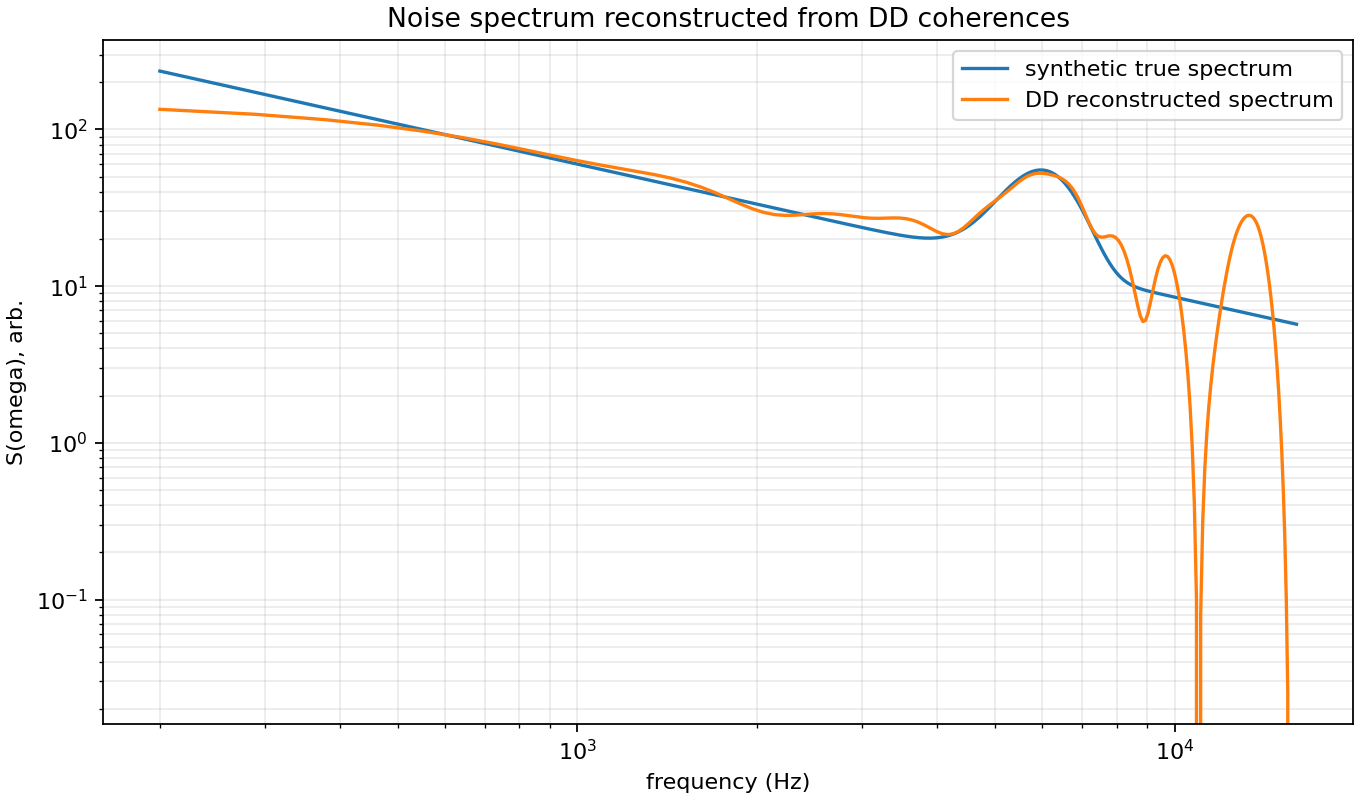
\includegraphics[width=0.82\textwidth]{../../outputs/workflows/experimental_decision_pipeline/latest/figures/reconstructed_noise_spectrum.png}
  }{
    \fbox{\parbox{0.82\textwidth}{Noise-spectrum figure not found. Run
    \texttt{python scripts/run\_experimental\_decision\_pipeline.py}.}}
  }
  \caption{Synthetic effective noise spectrum reconstructed from
  dynamical-decoupling coherence measurements.}
\end{figure}

\begin{figure}[ht]
  \centering
  \IfFileExists{../../outputs/workflows/experimental_decision_pipeline/latest/figures/control_sequence_decision.png}{
    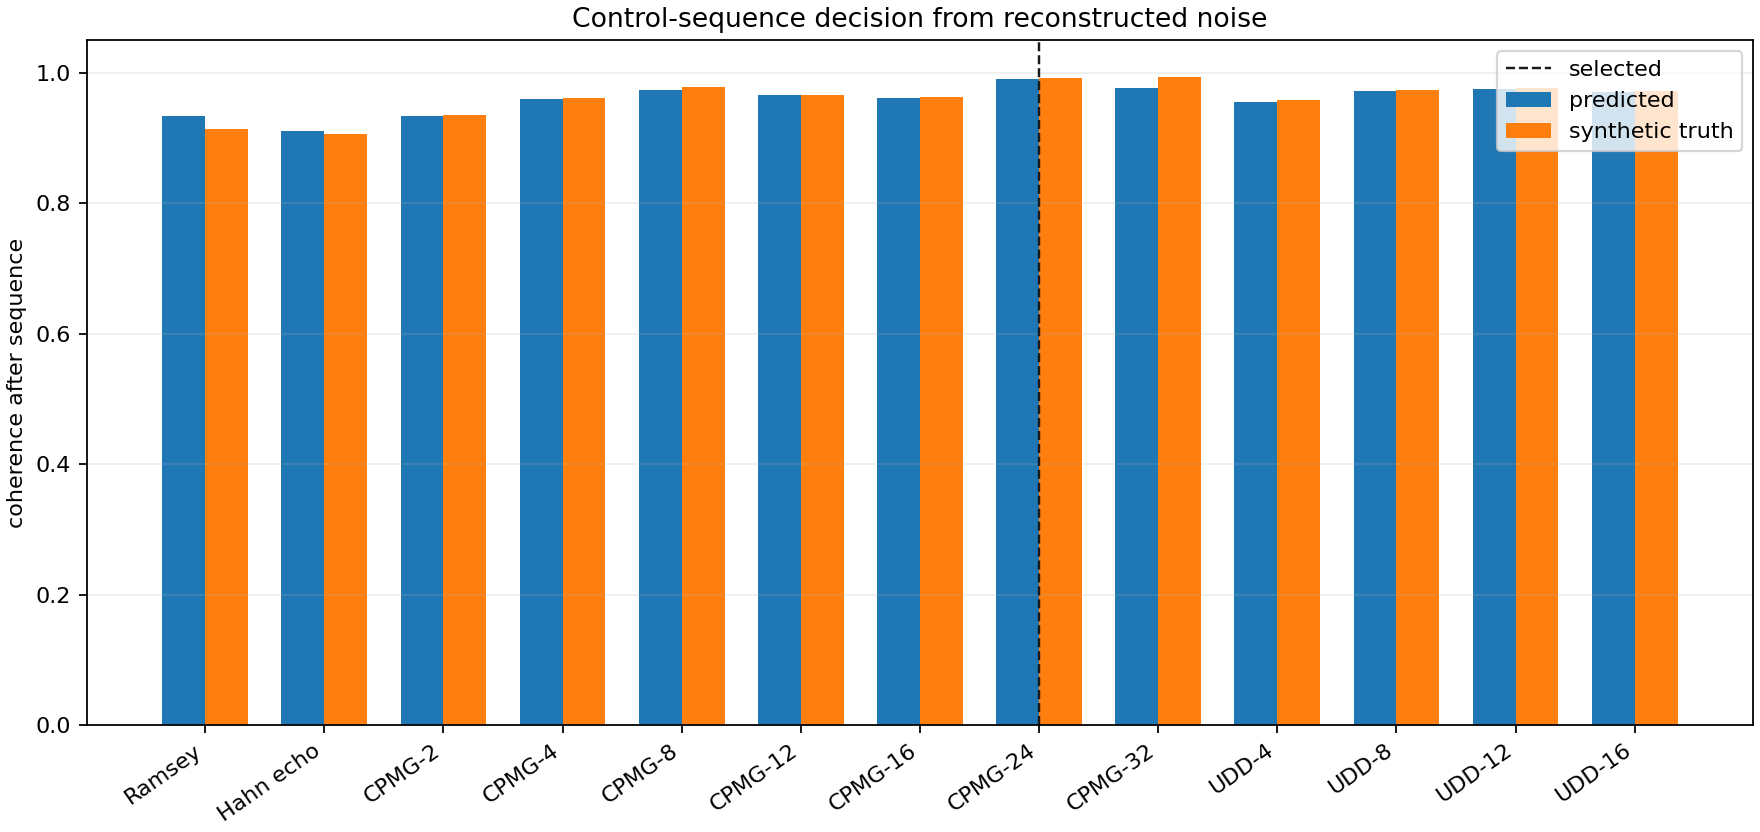
\includegraphics[width=0.82\textwidth]{../../outputs/workflows/experimental_decision_pipeline/latest/figures/control_sequence_decision.png}
  }{
    \fbox{\parbox{0.82\textwidth}{Control-decision figure not found. Run
    \texttt{python scripts/run\_experimental\_decision\_pipeline.py}.}}
  }
  \caption{Candidate control sequences scored by predicted coherence.}
\end{figure}

\section{What Can Be Claimed Now}

The current repository supports the following claims:
\begin{itemize}
  \item the Python spin-$3/2$ operator and Hamiltonian layer is internally
  validated by tests;
  \item the Na-23 FID and spectrum pipeline reproduces the expected central and
  satellite transition structure in the synthetic/reference setting;
  \item QST can reconstruct synthetic spin-$3/2$ density matrices and estimate
  relaxation rates under controlled assumptions;
  \item finite-pulse dynamics cannot be ignored for selective quadrupolar-NMR
  gates;
  \item optimal-control pulses are necessary for robust coherent operations in
  the encoded spin-$3/2$ manifold;
  \item DD filtering and DD spectroscopy provide a concrete route from
  coherence data to an effective noise spectrum;
  \item Markovian, GST, QPT, multipass-QPT, and process-tensor layers now exist
  as synthetic benchmarks for future hardware-facing characterization.
\end{itemize}

The current repository does not yet support these stronger claims:
\begin{itemize}
  \item that a real Na-23 sample follows the current synthetic relaxation
  model;
  \item that the selected CPMG-24 sequence is experimentally optimal;
  \item that a Lindblad model is sufficient for the real laboratory data;
  \item that hardware-level SPAM, pulse calibration, or readout errors have
  already been characterized.
\end{itemize}

\section{Failure Modes and Model Escalation}

The laboratory should treat disagreement with data as information, not as an
implementation failure.  The escalation logic is:
\begin{enumerate}
  \item If FID and spectrum peaks are shifted, inspect $\nu_Q$, offset, dwell
  time, phase convention, and apodization.
  \item If tomography residuals are large but spectra look reasonable, inspect
  pulse calibration, receiver phase, QST linear conditioning, and PSD projection.
  \item If DD coherences cannot be fitted by a positive spectrum, inspect pulse
  errors, relaxation channels beyond pure dephasing, and measurement
  uncertainty.
  \item If echo recovery or multi-time correlations disagree with a fixed
  Markovian model, escalate to memory-effective models or process tensors.
  \item If process reconstructions are non-physical, project onto the CPTP set
  or use constrained estimators.
  \item If gate errors are inseparable from SPAM, use GST-style predictive
  fitting rather than ordinary QPT alone.
\end{enumerate}

\section{Incoming Experimental Data Protocol}

When new lab data arrive, each run should provide:
\begin{itemize}
  \item raw data path and immutable copy;
  \item experiment identifier, date, operator, sample/device identifier;
  \item pulse sequence definitions and calibration values;
  \item dwell time, scans/shots, receiver phase, and preprocessing convention;
  \item uncertainty estimate for every coherence, spectrum, or tomography datum;
  \item comparison manifest filled from
  \texttt{lab\_manifest\_template.json};
  \item model snapshot and configuration hash.
\end{itemize}

The default operational question is:
\begin{quote}
Does the current synthetic-to-effective model predict the measured coherences
and QST observables within uncertainty?  If yes, use the selected control
sequence.  If no, identify which assumption failed and escalate the model
class.
\end{quote}

\section{Conclusion}

The current work has converted an initial MATLAB-based Na-23 NMR project into a
Python-first computational research laboratory.  The repository now contains a
validated spin-$3/2$ model, a reproducible set of paper-inspired benchmarks, a
research-memory agent, and an experimental-decision pipeline.  The main
scientific value is not any single synthetic number.  The value is the structure:
each claim is tied to code, configuration, metrics, figures, and tests.  This is
the foundation required to turn incoming NMR and quantum-hardware data into
defensible physical conclusions.

\appendix

\section{Commands}

\begin{verbatim}
cd <repo-root>
$env:PYTHONPATH='src'
python -m pytest -q
python scripts\run_experimental_decision_pipeline.py
python scripts\research_memory_agent.py
\end{verbatim}

\section{Artifact Locations}

\begin{verbatim}
outputs/repro/<paper_id>/latest/
outputs/workflows/experimental_decision_pipeline/latest/
lab/research_memory/
reports/review_article/
\end{verbatim}

\input{generated/complete_figure_atlas.tex}

\section{Bibliography}

\begin{thebibliography}{99}

\bibitem{na23_relaxometry_2023}
23Na relaxometry: An overview of theory and applications.
\emph{Magnetic Resonance Letters}, 2023.
doi:10.1016/j.mrl.2023.04.001.

\bibitem{spin32_algebraic_2004}
Algebraic description of spin 3/2 dynamics in NMR experiments.
\emph{Journal of Magnetic Resonance} 173(2), 236--253, 2005.
doi:10.1016/j.jmr.2004.12.009.

\bibitem{qst_relaxation_2008}
A study of the relaxation dynamics in a quadrupolar NMR system using Quantum
State Tomography.
\emph{Journal of Magnetic Resonance}, 2008.
doi:10.1016/j.jmr.2008.01.009.

\bibitem{spin32_qlogic_qst_2005}
Quantum logical operations for spin 3/2 quadrupolar nuclei monitored by quantum
state tomography.
\emph{Journal of Magnetic Resonance}, 2005.
doi:10.1016/j.jmr.2005.04.009.

\bibitem{nonmarkov_noise_2022}
Characterization and control of non-Markovian quantum noise.
\emph{Nature Reviews Physics}, 2022.
doi:10.1038/s42254-022-00446-2.

\bibitem{multipass_qpt_2024}
Multipass quantum process tomography.
\emph{Scientific Reports} 14, 18185, 2024.
doi:10.1038/s41598-024-68353-3.

\bibitem{quadrupolar_qip_2012}
Quantum information processing by nuclear magnetic resonance on quadrupolar
nuclei.
\emph{Philosophical Transactions of the Royal Society A} 370, 4770--4793, 2012.
doi:10.1098/rsta.2011.0365.

\bibitem{grape_nmr_control_2005}
Optimal control of coupled spin dynamics: Design of NMR pulse sequences by
gradient ascent algorithms.
\emph{Journal of Magnetic Resonance} 172(2), 296--305, 2005.
doi:10.1016/j.jmr.2004.11.004.

\bibitem{pps_optimal_control_2012}
Preparing Pseudo-Pure States in a Quadrupolar Spin System Using Optimal Control.
\emph{Chinese Physics Letters} 29(12), 127601, 2012.
doi:10.1088/0256-307X/29/12/127601.

\bibitem{projected_ls_qpt_2022}
Projected Least-Squares Quantum Process Tomography.
\emph{Quantum} 6, 844, 2022.
doi:10.22331/q-2022-10-20-844.

\bibitem{gst_2021}
Gate Set Tomography.
\emph{Quantum} 5, 557, 2021.
doi:10.22331/q-2021-10-05-557.

\bibitem{process_tensor_2020}
Demonstration of non-Markovian process characterisation and control on a quantum
processor.
\emph{Nature Communications} 11, 5301, 2020.
doi:10.1038/s41467-020-20113-3.

\bibitem{noise_filtering_2014}
Experimental noise filtering by quantum control.
\emph{Nature Physics} 10, 644--648, 2014.
doi:10.1038/nphys3115.

\bibitem{dd_noise_spectroscopy_2011}
Measuring the spectrum of colored noise by dynamical decoupling.
\emph{Physical Review Letters} 107, 230501, 2011.
doi:10.1103/PhysRevLett.107.230501.

\bibitem{flux_qubit_noise_2011}
Noise spectroscopy through dynamical decoupling with a superconducting flux
qubit.
\emph{Nature Physics} 7, 565--570, 2011.
doi:10.1038/nphys1994.

\end{thebibliography}

\end{document}
